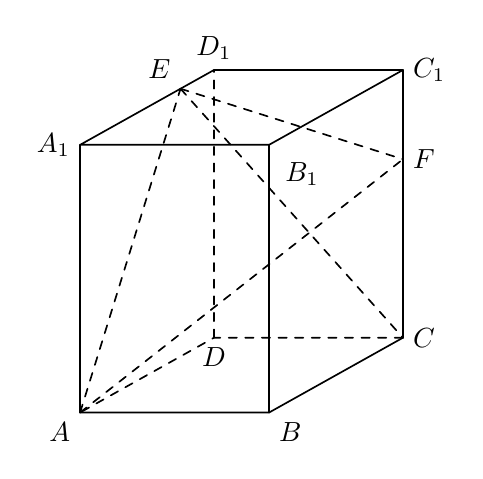
\begin{tikzpicture}[line width=.6pt,line join=round,line cap=round]
% oblique projection of cuboid ABCD-A1B1C1D1; front face true rectangle
\coordinate (A) at (0,0);
\coordinate (B) at (2.4,0);
\coordinate (D) at (1.7,0.95);
\coordinate (C) at (4.1,0.95);
\coordinate (A1) at (0,3.4);
\coordinate (B1) at (2.4,3.4);
\coordinate (D1) at (1.7,4.35);
\coordinate (C1) at (4.1,4.35);
\coordinate (E) at (1.275,4.1125);
\coordinate (F) at (4.1,3.2167);
% visible box edges (solid)
\draw (A) -- (B) -- (C);
\draw (A) -- (A1);
\draw (B) -- (B1);
\draw (C) -- (C1);
\draw (A1) -- (B1) -- (C1) -- (D1) -- cycle;
% hidden box edges (dashed)
\draw[dashed] (C) -- (D) -- (A);
\draw[dashed] (D) -- (D1);
% interior diagonals (all dashed as in original)
\draw[dashed] (A) -- (E);
\draw[dashed] (A) -- (F);
\draw[dashed] (E) -- (F);
\draw[dashed] (E) -- (C);
% labels placed tight to points, clear of edges
\node[below left,font=\normalsize] at (A) {$A$};
\node[below right,font=\normalsize] at (B) {$B$};
\node[right,font=\normalsize] at (C) {$C$};
\node[below,font=\normalsize] at (D) {$D$};
\node[left,font=\normalsize] at (A1) {$A_1$};
\node[anchor=north west,font=\normalsize] at ([shift={(0.08,-0.10)}]B1) {$B_1$};
\node[right,font=\normalsize] at (C1) {$C_1$};
\node[above,font=\normalsize] at (D1) {$D_1$};
\node[above left,font=\normalsize] at (E) {$E$};
\node[right,font=\normalsize] at (F) {$F$};
\end{tikzpicture}
